%%%%%%%%%%%%%%%%%%%%%%%%%%%%%%%%%%%%%%%%%%%%%%%%%%%%%%%%%%%%%%%%%%%%%%%%%%%%%%%%%%%%%%%%%%%%%%%%%%%%%%%%%%%%%%%%%%%%%%%%%%%%%%%%%%%%%%%%%%%%%%%%%%%%%%%%%%%%%%%%%%%%%%%
%%%%%%%%%%%%%%%%%%%%%%%%%%%%%%%%%%%%%%%%%%%%%%%%%%%%%%%%%%%%%%%%%%%%%%%%%%%%%%%%%%%%%%%%%%%%%%%%%%%%%%%%%%%%%%%%%%%%%%%%%%%%%%%%%%%%%%%%%%%%%%%%%%%%%%%%%%%%%%%%%%%%%%%
%%% Modèle pour la 4ème de couverture des thèses préparées à l'Institut Polytechnique de Paris, basé sur le modèle produit par Nikolas STOTT / Template for back cover of thesis made at Institut Polytechnique de Paris, based on the template made by Nikolas STOTT
%%% Mis à jour par Aurélien ARNOUX (École polytechnique)/ Updated by Aurélien ARNOUX (École polytechnique)
%%% Les instructions concernant chaque donnée à remplir sont données en bloc de commentaire / Rules to fill this file are given in comment blocks
%%% ATTENTION Ces informations doivent tenir sur une seule page une fois compilées / WARNING These informations must contain in no more than one page once compiled
%%%%%%%%%%%%%%%%%%%%%%%%%%%%%%%%%%%%%%%%%%%%%%%%%%%%%%%%%%%%%%%%%%%%%%%%%%%%%%%%%%%%%%%%%%%%%%%%%%%%%%%%%%%%%%%%%%%%%%%%%%%%%%%%%%%%%%%%%%%%%%%%%%%%%%%%%%%%%%%%%%%%%%%
%%% Version du 28 avril 2020 : utilisation de .png au lieu de .jpg pour les logos
%%%%%%%%%%%%%%%%%%%%%%%%%%%%%%%%%%%%%%%%%%%%%%%%%%%%%%%%%%%%%%%%%%%%%%%%%%%%%%%%%%%%%%%%%%%%%%%%%%%%%%%%%%%%%%%%%%%%%%%%%%%%%%%%%%%%%%%%%%%%%%%%%%%%%%%%%%%%%%%%%%%%%%%

% \documentclass[a4paper]{article}
% \usepackage[utf8]{inputenc}
% \usepackage{helvet}
% \renewcommand{\familydefault}{\sfdefault}
% \usepackage{geometry}
% \geometry{
% left=16mm,
% top=30mm,
% right=16mm,
% bottom=30mm
% }
% \usepackage{xcolor}
% \usepackage[absolute,overlay]{textpos}
% \usepackage{graphicx}
% \usepackage{lipsum}
% \usepackage{array}
% \usepackage{caption}
% \usepackage{multicol}
% \setlength{\columnseprule}{0pt}
% \setlength\columnsep{10pt}

% \usepackage[french]{babel}

\label{form2}
%%%%%%%%%%%%%%%%%%%%%%%%%%%%%%%%%%%%%%%%%%%%%%%%%%%%%%%%%%%%%%%%%%%%%%%%%%%%%%%%%%%%%%%%%%%%%%%%%%%%%%%%%%%%%%%%%%%%%%%%%%%%%%%%%%%%%%%%%%%%%%%%%%%%%%%%%%%%%%%%%%%%%%%
%%%%%%%%%%%%%%%%%%%%%%%%%%%%%%%%%%%%%%%%%%%%%%%%%%%%%%%%%%%%%%%%%%%%%%%%%%%%%%%%%%%%%%%%%%%%%%%%%%%%%%%%%%%%%%%%%%%%%%%%%%%%%%%%%%%%%%%%%%%%%%%%%%%%%%%%%%%%%%%%%%%%%%%
%%% Formulaire / Form
%%% Remplacer les paramètres des \newcommand par les informations demandées / Replace \newcommand parameters by asked informations
%%%%%%%%%%%%%%%%%%%%%%%%%%%%%%%%%%%%%%%%%%%%%%%%%%%%%%%%%%%%%%%%%%%%%%%%%%%%%%%%%%%%%%%%%%%%%%%%%%%%%%%%%%%%%%%%%%%%%%%%%%%%%%%%%%%%%%%%%%%%%%%%%%%%%%%%%%%%%%%%%%%%%%%
%%%%%%%%%%%%%%%%%%%%%%%%%%%%%%%%%%%%%%%%%%%%%%%%%%%%%%%%%%%%%%%%%%%%%%%%%%%%%%%%%%%%%%%%%%%%%%%%%%%%%%%%%%%%%%%%%%%%%%%%%%%%%%%%%%%%%%%%%%%%%%%%%%%%%%%%%%%%%%%%%%%%%%%


\newcommand{\logoEd}{ed}																		%% Logo de l'école doctorale. Indiquer le sigle (EDIPP, EDMH) / Doctoral school logo. Indicate the acronym : EDMH, EDIPP
\textblockcolor{white}
\newcommand{\PhDTitleFR}{Pour un internet des objets sécurisé et respectueux de la vie privée basé sur le contrôle d'usage et les registres distribués}													%% Titre de la thèse en français / Thesis title in french
\newcommand{\keywordsFR}{Internet des Objets, Systèmes distribués, Vie privée, Contrôle d'usage, RGPD}														%% Mots clés en français, séprarés par des , / Keywords in french, separated by ,
\newcommand{\abstractFR}{\lipsum[1-3]}															%% Résumé en français / abstract in french

\newcommand{\PhDTitleEN}{For a Private and Secure Internet of Things with Usage Control and Distributed Ledger Technology
}													%% Titre de la thèse en anglais / Thesis title in english
\newcommand{\keywordsEN}{Internet of Things, Distributed Systems, Privacy, Usage Control, GDPR}														%% Mots clés en anglais, séprarés par des , / Keywords in english, separated by ,
%\newcommand{\abstractEN}{\lipsum[1-3]}															%% Résumé en anglais / abstract in english

% \label{layout}
%%%%%%%%%%%%%%%%%%%%%%%%%%%%%%%%%%%%%%%%%%%%%%%%%%%%%%%%%%%%%%%%%%%%%%%%%%%%%%%%%%%%%%%%%%%%%%%%%%%%%%%%%%%%%%%%%%%%%%%%%%%%%%%%%%%%%%%%%%%%%%%%%%%%%%%%%%%%%%%%%%%%%%%
%%%%%%%%%%%%%%%%%%%%%%%%%%%%%%%%%%%%%%%%%%%%%%%%%%%%%%%%%%%%%%%%%%%%%%%%%%%%%%%%%%%%%%%%%%%%%%%%%%%%%%%%%%%%%%%%%%%%%%%%%%%%%%%%%%%%%%%%%%%%%%%%%%%%%%%%%%%%%%%%%%%%%%%
%%% Mise en page / Page layout      
%%% NE RIEN MODIFIER / DO NOT MODIFY
%%%%%%%%%%%%%%%%%%%%%%%%%%%%%%%%%%%%%%%%%%%%%%%%%%%%%%%%%%%%%%%%%%%%%%%%%%%%%%%%%%%%%%%%%%%%%%%%%%%%%%%%%%%%%%%%%%%%%%%%%%%%%%%%%%%%%%%%%%%%%%%%%%%%%%%%%%%%%%%%%%%%%%%
%%%%%%%%%%%%%%%%%%%%%%%%%%%%%%%%%%%%%%%%%%%%%%%%%%%%%%%%%%%%%%%%%%%%%%%%%%%%%%%%%%%%%%%%%%%%%%%%%%%%%%%%%%%%%%%%%%%%%%%%%%%%%%%%%%%%%%%%%%%%%%%%%%%%%%%%%%%%%%%%%%%%%%%

% \begin{document}
\pagestyle{empty}

%%% Logo de l'école doctorale. Le nom du fichier correspond au sigle de l'ED / Doctoral school logo. Filename correspond to doctoral school acronym
%%% Les noms valides sont / Valid names are : EDMH, (EDIPP)
\begin{textblock*}{61mm}(16mm,3mm)
	\noindent
\includegraphics[height=24mm]{media/ed/EDIPP-en.png}
\end{textblock*}



%%%Titre de la thèse en français / Thesis title in french
\begin{center}
\fcolorbox{black}{white}{\parbox{0.99\textwidth}{
{\bf Titre:} \PhDTitleFR 
\medskip

%%%Mots clés en français, séprarés par des ; / Keywords in french, separated by ;
{\bf Mots clés:} \keywordsFR 
\vspace{-2mm}

%%% Résumé en français / abstract in french
\begin{multicols}{2}
{\bf Résumé:} 
Les objets connectés représentent l'une des principales cibles de la cybercriminalité. Les raisons en sont multiples : d'abord, pour des raisons commerciales, les fabricants peuvent vendre des produits vulnérables qui posent des problèmes de sécurité. Deuxièmement, de nombreux appareils IoT sont soumis à des contraintes de performance et ne disposent pas de la puissance nécessaire pour exécuter des logiciels de sécurité. Enfin, l'hétérogénéité des applications, du matériel et des logiciels élargit la surface d'attaque.
Pour parer à ces menaces, l'IoT a besoin de technologies de sécurité et de préservation de la vie privée sur mesure.

 En ce qui concerne la protection de la vie privée, \emph{le contrôle d'usage} donne aux utilisateurs la possibilité de spécifier comment leurs données peuvent être utilisées et par qui. Le contrôle d'usage étend le contrôle d'accès classique en introduisant des \emph{obligations}, c'est-à-dire des actions à effectuer pour obtenir l'accès, et des \emph{conditions} qui sont liées à l'état du système, comme la charge du réseau ou le temps.
Cette thèse vise à apporter des réponses aux défis de l'internet des objets en termes de performance, de sécurité et de respect de la vie privée. Pour cela, les registres distribués (DLT) constituent une solution prometteuse aux contraintes de l'internet des objets, en particulier pour les micro-transactions, notamment par leur caractère décentralisé. Cela se traduit par trois contributions:
1. un ensemble de technologies pour des transactions sans frais préservant la vie privée, conçu pour passer à l'échelle;
2. une méthode d'intégration du contrôle d'usage et des registres distribués pour permettre une protection efficace des données des utilisateurs;
3. un modèle étendu pour le contrôle d'usage dans les systèmes distribués, afin d'y ajouter le contrôle de flux décentralisé et les aspects liés à l'internet des objets.
Une preuve de concept de l'intégration (2) a été mise en place pour démontrer la faisabilité et effectuer des tests de performance. Il s'appuie sur IOTA, un registre distribué qui utilise un graphe orienté acyclique pour son graphe de transactions au lieu d'une \emph{blockchain}. Les résultats des tests de performance sur un réseau privé montrent une diminution d'environ 90\% du temps nécessaire pour effectuer des transactions et pour évaluer des politiques de contrôle d'usage, dans le cas où ce dernier est intégré au réseau.
\end{multicols}
}}
\end{center}

\vspace*{0mm}

%%%Titre de la thèse en anglais / Thesis title in english
\begin{center}
\fcolorbox{black}{white}{\parbox{0.99\textwidth}{
{\bf Title: } \PhDTitleEN 

\medskip

%%%Mots clés en anglais, séprarés par des ; / Keywords in english, separated by ;
{\bf Keywords:}  \keywordsEN %%3 à 6 mots clés%%
\vspace{-2mm}
\begin{multicols}{2}
	
%%% Résumé en anglais / abstract in english
{\bf Abstract:} 

IoT devices represent one of the major targets for malicious activities. The grounds for this are manifold: first, to reduce the cost of security, manufacturers may sell vulnerable products, leaving users with security concerns. Second, many IoT devices have performance constraints and lack the processing power to execute security software. Third, the heterogeneity of applications, hardware, and software widens the attack surface.
As a result, IoT networks are subject to a variety of cyber threats. To counter such a variety of attacks, the IoT calls for security and privacy-preserving technologies.
%Solutions
 For privacy concerns, \emph{usage control} grants the users the power to specify how their data can be used and by whom. Usage control extends classic access control by introducing \emph{obligations}, i.e., actions to be performed to be granted access, and \emph{conditions} that are related to the system state, such as the network load or the time.
%Main contributions

This thesis aims at providing answers to the challenges in the Internet of Things in terms of performance, security and privacy. To this end, \emph{distributed ledger technologies} (DLTs) are a promising solution to Internet of Things constraints, in particular for micro-transactions, due to the decentralization they provide. This leads to three related contributions:
1. a framework for zero-fee privacy-preserving transactions in the Internet of Things designed to be scalable;
2. an integration methodology of usage control and distributed ledgers to enable efficient protection of users' data;
3. an extended model for data usage control in distributed systems, to incorporate decentralized information flow control and IoT aspects.
A proof of concept of the integration (2) has been designed to demonstrate feasibility and conduct performance tests. It is based on IOTA, a distributed ledger using a directed acyclic graph for its transaction graph instead of a blockchain. The results of the tests on a private network
show an approximate 90\% decrease in the time needed to push transactions
and make access decisions in the integrated setting.
\end{multicols}
}}
\end{center}


\begin{textblock*}{161mm}(10mm,270mm)
\color{black}
\textblockcolor{white}
{\bf\noindent Institut Polytechnique de Paris	         }

\noindent
\noindent 91120 Palaiseau, France 
\end{textblock*}

\begin{textblock*}{20mm}(175mm,265mm)
\textblockcolor{white}
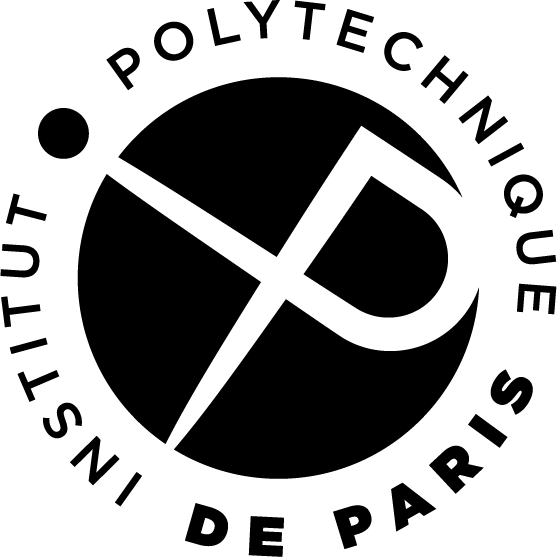
\includegraphics[width=20mm]{media/IPPARIS-petit}
\end{textblock*}

% \end{document}